\documentclass[11pt]{scrartcl}
\usepackage[utf8]{inputenc}
\usepackage{enumitem}
\usepackage{amsfonts}
\usepackage{bbm}
\usepackage{newtxmath}
%\usepackage[square]{natbib}
\usepackage{amsmath}
\usepackage{mathrsfs,bm}
\usepackage{graphicx,epstopdf,caption}
\usepackage{float,subcaption,setspace,booktabs,multirow,supertabular,lscape,threeparttable}
\usepackage{float,colortbl}
\usepackage{placeins}
\usepackage{indentfirst}
\usepackage{enumitem}
\setlength{\parindent}{0pt} %% noindent for the entire file % or add indent {2em}
\usepackage{geometry}
\geometry{left=0.8in,right=0.8in,top=1in,bottom=0.5in}
\usepackage[noblocks]{authblk}
\usepackage{lipsum}%% a garbage package you don't need except to create examples.
\usepackage{fancyhdr}
\usepackage[svgnames]{xcolor}
\usepackage{listings}
\usepackage{verbatim}
\usepackage[round, semicolon, sort]{natbib}
\setlength{\parindent}{2em}
\usepackage[font={footnotesize, it}]{caption}

\pagestyle{fancy}
\lhead{CSCI 5561}  % set your name here
\chead{\large\textbf{Homework 2 - Registration}}
\rhead{He Zhou (zhou1354@umn.edu)}
\renewcommand{\headrulewidth}{0.4pt}

\lstset{language=R,
	basicstyle=\small\ttfamily,
	stringstyle=\color{DarkGreen},
	otherkeywords={0,1,2,3,4,5,6,7,8,9},
	morekeywords={TRUE,FALSE},
	deletekeywords={data,frame,length,as,character},
	keywordstyle=\color{blue},
	commentstyle=\color{DarkGreen},
}
\usepackage{Sweave}
\graphicspath{{Figures/}}  % set the path of figures
\usepackage{blindtext}
\usepackage{scrextend}
\addtokomafont{labelinglabel}{\bfseries}
\usepackage{appendix}
\usepackage[linesnumbered,ruled,vlined]{algorithm2e}

\usepackage{algpseudocode}  
\usepackage{hyperref}
\hypersetup{
    colorlinks=true,
    linkcolor=blue,
    filecolor=blue,      
    urlcolor=blue,
    citecolor=cyan,
}

\newcommand{\cX}{\mathcal{X}}
\newcommand{\cR}{\mathcal{R}}
\newcommand{\cV}{\mathcal{V}}
\newcommand{\bw}{\mathbf{w}}

	

\begin{document}

\title{CSCI 5561}
\author{\Large Homework 2 -- Registration\\
	He Zhou}  %% set your name on the main page
%\date{\vspace{-5ex}}  % suppress the output of date
\maketitle

\newpage
\paragraph{\textbf{SIFT Feature Extration:}}
Given an image (1a), we use \texttt{OpenCV} library to extract SIFT features. Image (1b) shows the keypoints with the circles of their size and their orientations.


\begin{figure}[H]
	\captionsetup[subfigure]{labelformat=empty}
	\centering
	\subcaptionbox{(1a) Image frame 1}{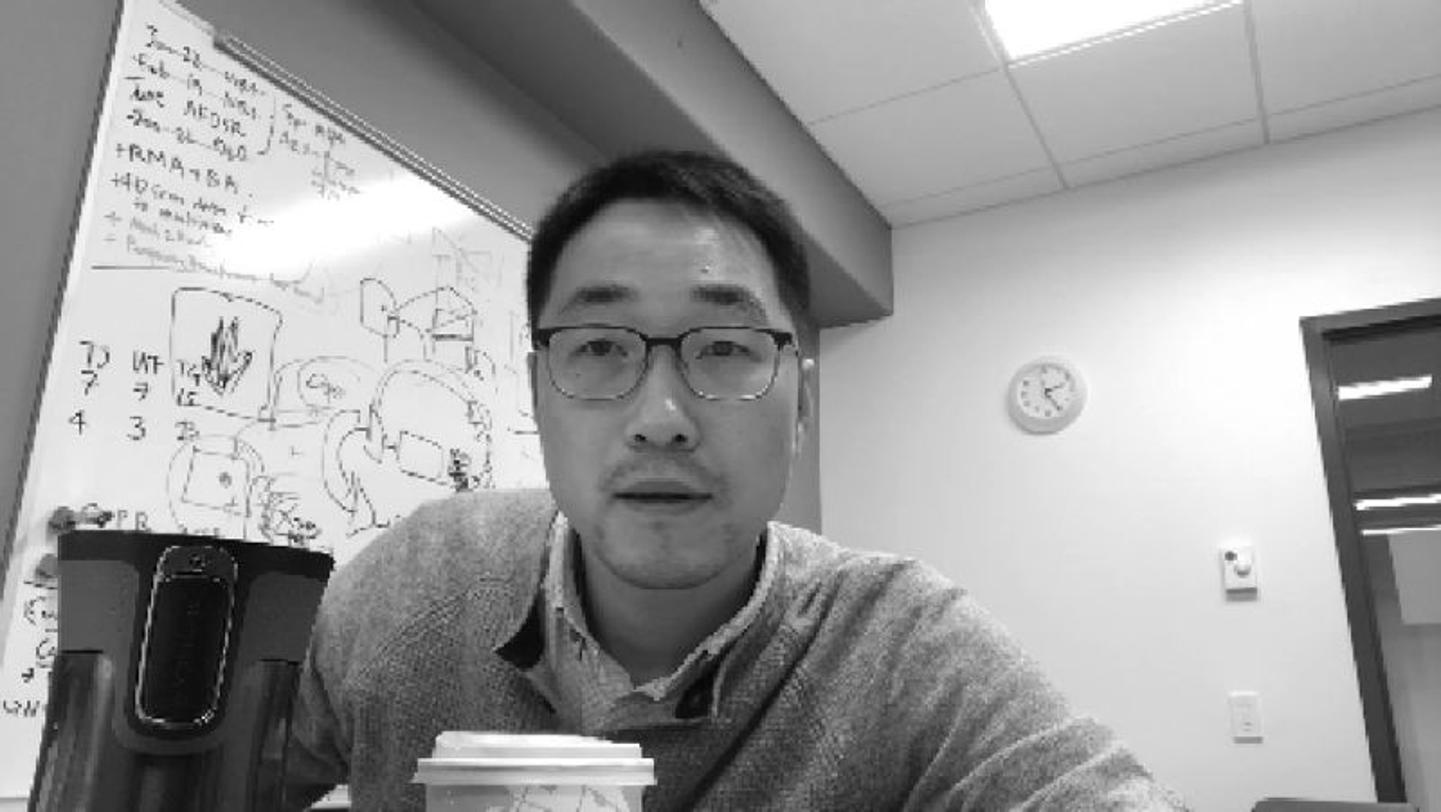
\includegraphics[height=3cm,keepaspectratio]{Hyun_Soo_target1.jpg}}
	\subcaptionbox{(1b) SIFT}{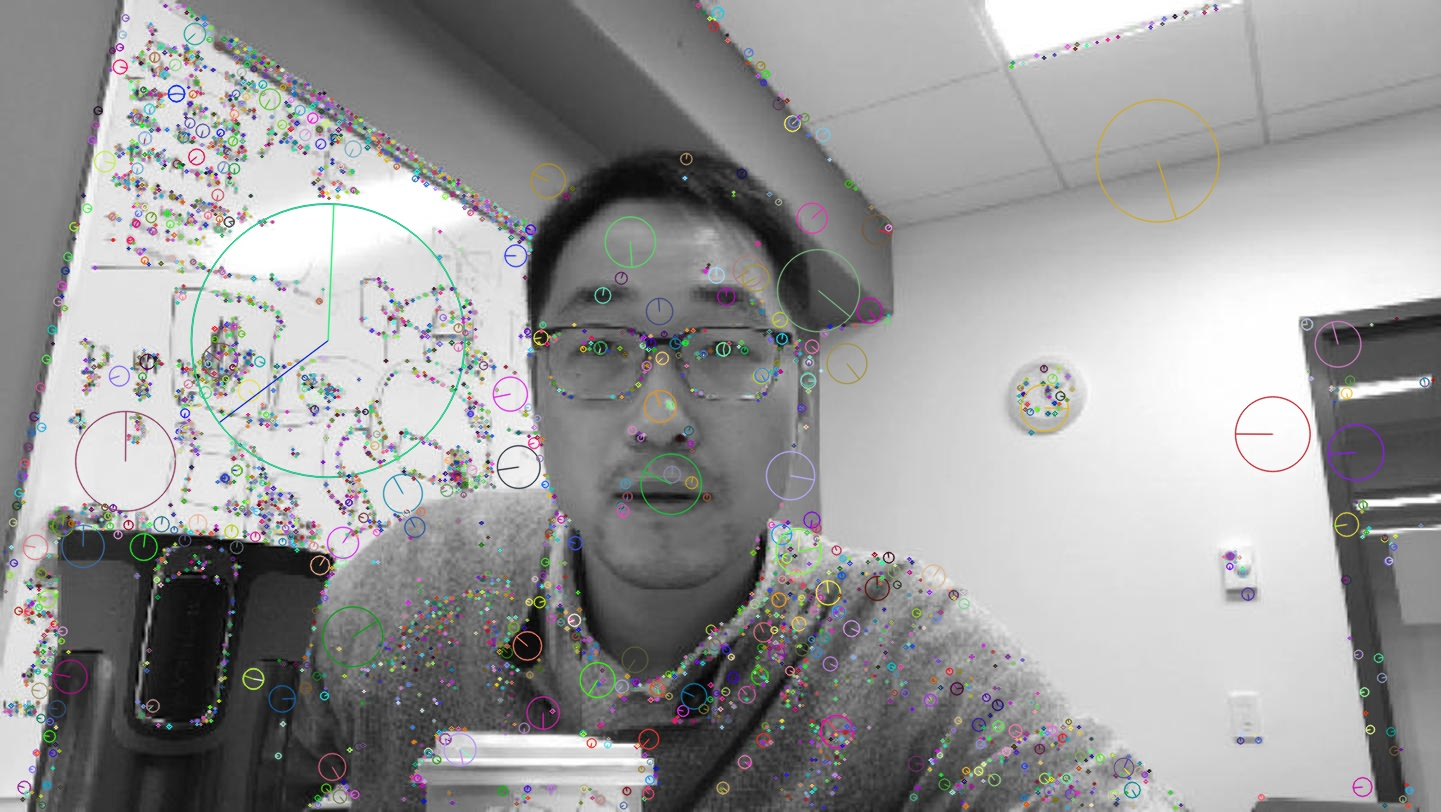
\includegraphics[height=3cm,keepaspectratio]{sift_keypoints_target1.jpg}}
	\label{fig:SIFT}
\end{figure}

\paragraph{\textbf{SIFT Feature Matching:}} 
We use the SIFT features to match between the template image and the target image. In specific, use two sets of keypoint descriptors / SIFT features from the template and target, find the matches using nearest neighbor with the ratio test, i.e., take the ratio of distances of first nearest neighbor and second nearest neighbor and drop those with ratio $\geq 0.7$. Threshold $0.7$ is chosen empirically to control the type I and type II errors simultaneously. Image (2a) and (2b) show the template and target image. Image (2c) shows the matching points between the template and the target. We can see most of the matches are correct but their are some noisy matches.


\begin{figure}[H]
	\captionsetup[subfigure]{labelformat=empty}
	\centering
	\subcaptionbox{(2a) Template}{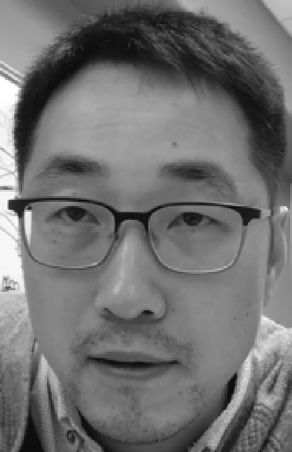
\includegraphics[height=3cm,keepaspectratio]{Hyun_Soo_template.jpg}}
	\subcaptionbox{(2b) Target}{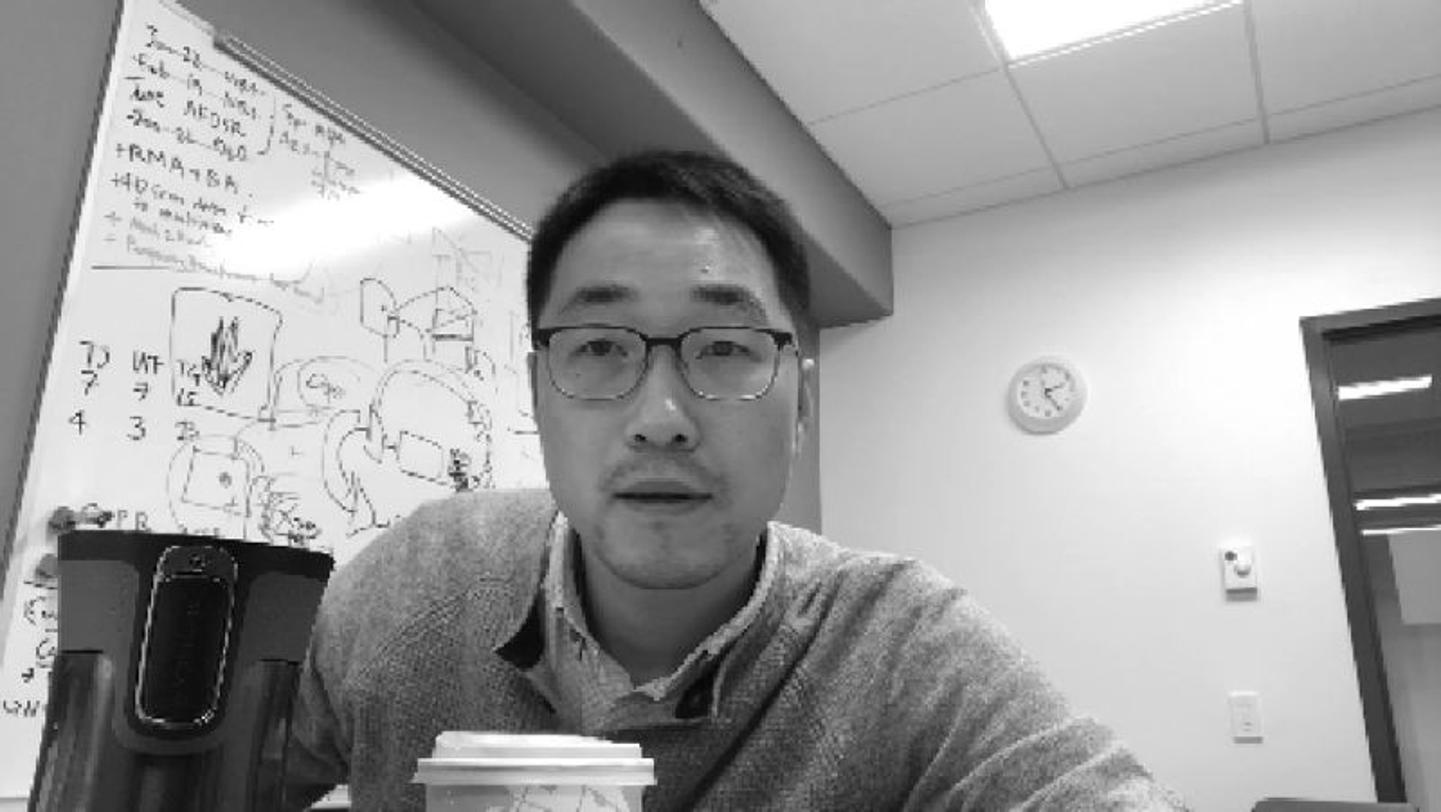
\includegraphics[height=3cm,keepaspectratio]{Hyun_Soo_target1.jpg}}
	\subcaptionbox{(2c) SIFT matches with ratio test}{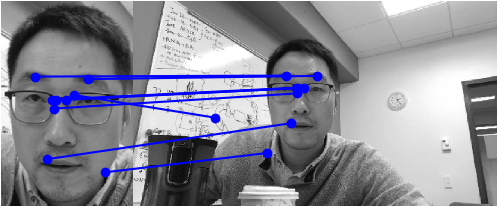
\includegraphics[height=3cm,keepaspectratio]{sift_match_target1.png}}
	\label{fig:SIFT_match}
\end{figure}

\paragraph{\textbf{Feature-based Image Alignment:}} 
The noisy SIFT matches can be filtered by RANSAC with an affine transformation. Since affine transformation has $6$ degrees of freedom, we need $3$ pairs of correspondences in SIFT matches to determine it. The RANSAC procedues are as follow: We randomly sample $3$ pairs of SIFT matches, determine the affine transformation, project the keypoints in template to the target domain, calculate the Euclidean distance between the projected points and matched points, and find the inliers based on a given thresholds (\texttt{ransac\_thr=10}). The whole procedure is repeated $\texttt{ransac\_iter}=1000$ times (with the random seed set as $5561$ for reproducibility). The transformation that gives the maximum number of inliers is chosen. Figure (3a) shows the projection of the template into the target domain using the RANSAC-filtered affine transformation. 

\paragraph{\textbf{Image Warping:}}
Use the affine transform to warp the target image to the template using the inverse mapping. The inverse mapping method is applied to make sure the warped image does not produce empty pixel. For each pixel in the output image \texttt{img\_warped}, project onto the domain of the input image \texttt{img} using the affine transformation \texttt{A}, then use bilinear interpolation to determine its value based on the input image \texttt{img}. We use \texttt{interpn} function imported from \texttt{scipy.interpolate} for bilinear interpolation. Figure (3c) shows the warped image. Figure (3d) shows the error map $\vert I_{\text{tpl}}-I_\text{wrp}\vert$.




\begin{figure}[H]
	\captionsetup[subfigure]{labelformat=empty}
	\centering
	\subcaptionbox{(3a) Red: Boundary of the transformed template.}{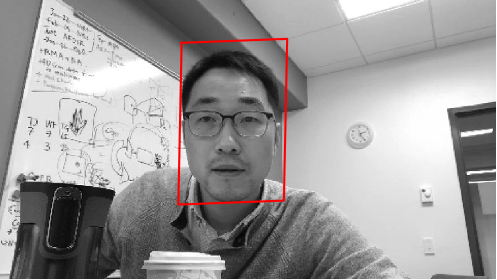
\includegraphics[height=3cm,keepaspectratio]{initial_boundary_target1.png}}
	\subcaptionbox{(3b) Template}{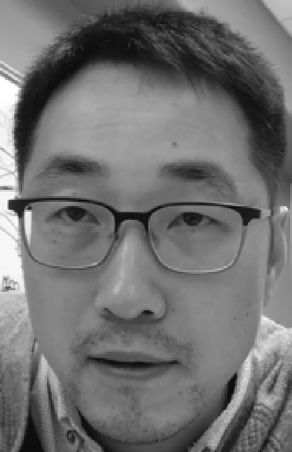
\includegraphics[height=3cm,keepaspectratio]{Hyun_Soo_template.jpg}}
	\subcaptionbox{(3c) Warped image}{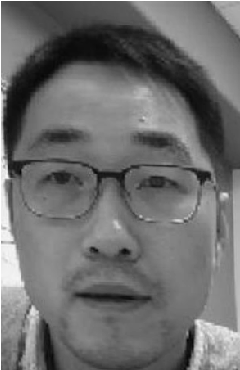
\includegraphics[height=3cm,keepaspectratio]{initial_warped_target1.png}}
	\subcaptionbox{(3d) Error map}{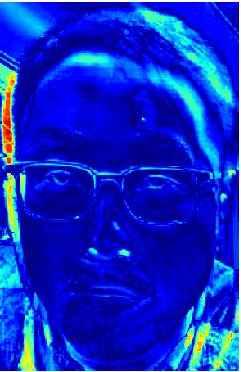
\includegraphics[height=3cm,keepaspectratio]{initial_error_target1.png}}
\end{figure}



\paragraph{\textbf{Inverse Compositional Image Alignment (ICIA):}}
Given the initial estimate of the affine transform from the feature based image alignment, we can track the next frame image using the inverse compositional method. We reparametrize the affine tramsform and refine the affine transform using inverse compositonal image alignment. Image (4a) shows the template image \texttt{`Hyun\_Soo\_template.jpg'} for the first frame image. Image (4b) shows the first frame image with the initialization of the affine transform from the feature based image alignment. Image (4c) shows the optimized affine transform using ICIA. Figure (4d) shows the comparison of the initial warp and optimized warp for frame image 1. Figure (4e) shows the error plot over iterations.




\begin{figure}[H]
	\captionsetup[subfigure]{labelformat=empty}
	\centering
	\subcaptionbox{(4a) Template}{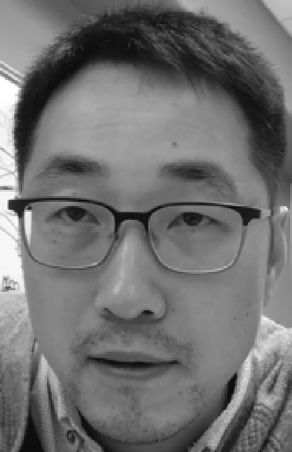
\includegraphics[height=3cm,keepaspectratio]{Hyun_Soo_template.jpg}}
	\subcaptionbox{(4b) Initialization for target1}{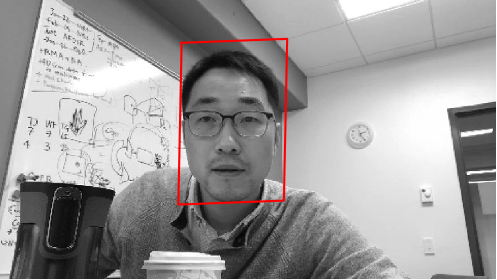
\includegraphics[height=3cm,keepaspectratio]{initial_boundary_target1.png}}
	\subcaptionbox{(4c) ICIA for target1 }{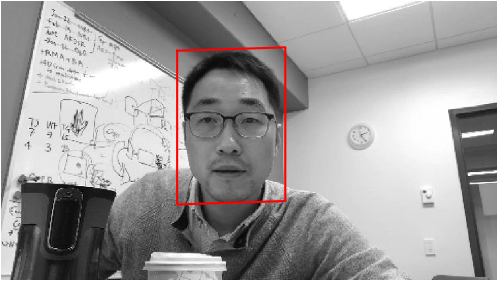
\includegraphics[height=3cm,keepaspectratio]{aligned_target1.png}}
	\subcaptionbox{(4d) Template for target1}{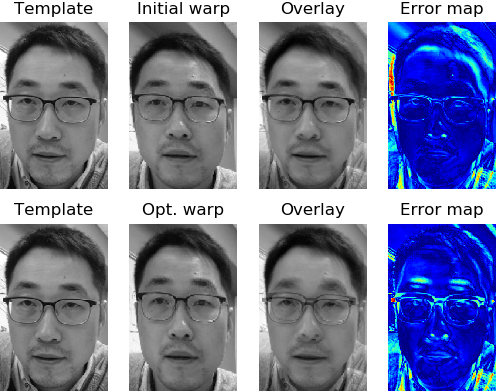
\includegraphics[height=4cm,keepaspectratio]{ICIA_target1.png}}
	\subcaptionbox{(4e) Error plot}{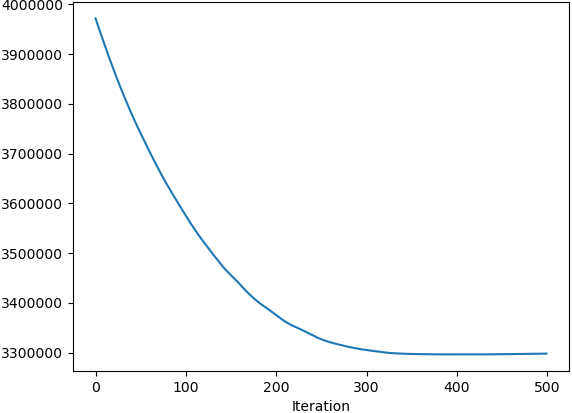
\includegraphics[height=3cm,keepaspectratio]{ICIA_errors_target1.png}}
\end{figure}



\paragraph{\textbf{Putting Things Together: Multiframe Tracking}}
Given a template and a set of consecutive images, we will first initialize the affine transform using the featured based alignment and then track over frames using the inverse compositonal image alignment. The template image is updated at every frame, i.e., the ICA-warped image of frame image 1 will be used as the template for frame image 2, and so on so forth. The initial transform is set as the refined transform of the previous step.

\begin{figure}[H]
	\captionsetup[subfigure]{labelformat=empty}
	\centering
	\subcaptionbox{(5a) Template }{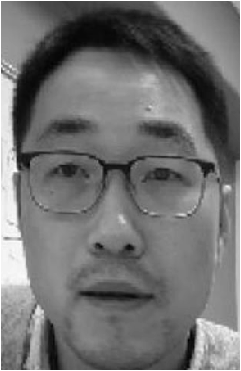
\includegraphics[height=2.8cm,keepaspectratio]{template_for_target2.png}}
	\subcaptionbox{(5b) Initialization for target2}{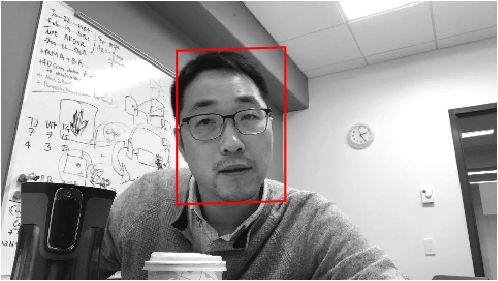
\includegraphics[height=2.8cm,keepaspectratio]{initial_target2.png}}
	\subcaptionbox{(5c) ICIA for target2}{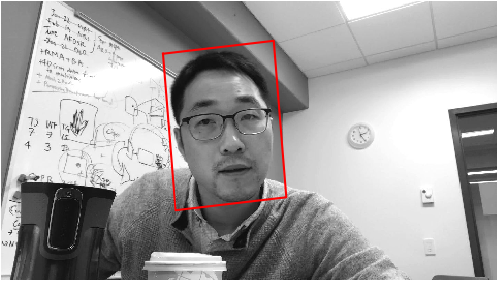
\includegraphics[height=2.8cm,keepaspectratio]{aligned_target2.png}}
	\subcaptionbox{(5d) Comparison for target2}{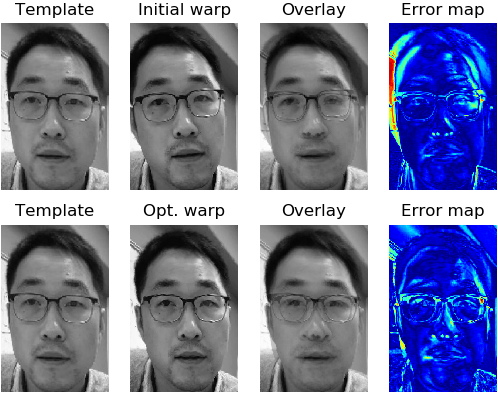
\includegraphics[height=2.8cm,keepaspectratio]{ICIA_target2.png}}
\end{figure}




\begin{minipage}{0.45\textwidth}
	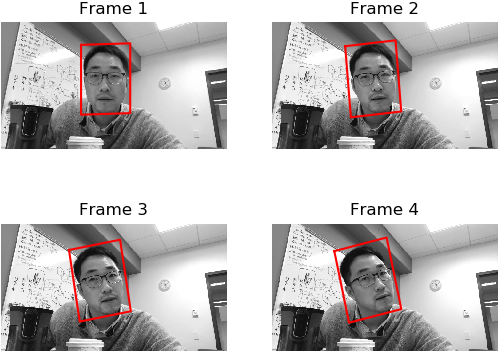
\includegraphics[width=0.9\linewidth]{ICIA_track.png}
\end{minipage}
\begin{minipage}{0.5\textwidth}\raggedright
	\quad Image (5a) shows the aligned image from the frame image 1 as the template for frame image 2. Image (5b) shows the initialization of the affine transform for the frame image 2. Image (5c) shows the optimized affine transform using ICIA. Image (5d) shows the comparison between initial and optimized transform.
	\\
	\quad This left figure shows the tracking of the frames for four consecutive images using ICIA.
\end{minipage}










\nocite*{}  
%\bibliographystyle{apalike}  %disordered
%\bibliographystyle{plain}  %ordered by auther
%\bibliographystyle{unsrt}  %ordered as referenced
\bibliographystyle{IEEEtranN}
\bibliography{bibfile}






\end{document}